\section{Calculation of Relative Entropy}
\subsection{Pure-Pure}
We calculate now the quantum relative entropy of two states of the type \eqref{condentpsi} to make a somewhat general calculation with arbitrary parameters. Let the parameters be $0<u,v<\pi/2$,
hence the density matrices are $\sigma_u=\ket{\psi(u)}\bra{\psi(u)}$ and $\sigma_v=\ket{\psi(v)}\bra{\psi(v)}$. The eigendecomposition is identical to the calculation of section \ref{sectioncondcalc} thus we have all the expressions needed for our calculations.
We will calculate $Q(\sigma_u \| \sigma_v)$ but it is obviously symmetric under the interchange of variables $u$ and $v$. 

\begin{align}
Q(\sigma_u \| \sigma_v) &=S(\sigma_u)-\lim_{\epsilon \to -\infty} \left\{ \Tr \left[
\sigma_u M_v
\left(
\begin{array}{cccc}
 G(\epsilon;1) & 0 & 0 & 0 \\
 0 &  G(\epsilon;0) & 0 & 0 \\
 0 & 0 &  G(\epsilon;0) & 0 \\
 0 & 0 & 0 &  G(\epsilon;0) \\
\end{array}
\right) M_v^{-1} \right] \right\} \nonumber \\[0.5em]
&= -\lim_{\epsilon \to -\infty} \left\{ \Tr \left[ \sigma_u
\left(
\begin{array}{cccc}
 \epsilon  \sin ^2(v) & 0 & 0 & -\epsilon  \cos (v) \sin (v) \\
 0 & \epsilon  & 0 & 0 \\
 0 & 0 & \epsilon  & 0 \\
 -\epsilon  \cos (v) \sin (v) & 0 & 0 & \epsilon  \cos ^2(v) \\
\end{array}
\right)
 \right] \right\} \nonumber \\[0.5em]
&=-\lim_{\epsilon \to -\infty} \left( \epsilon  \sin ^2(v-u) \right) \nonumber \\[0.5em]
&=
\begin{cases}
   +\infty   &   u \neq v\\
   0  &   u=v
\end{cases}
\end{align}
This result is expected. Different pure states diverge while quantum relative entropy is zero the matrix arguments are identical.
\subsection{Mixed-Mixed}
We now calculate an example of a mixed vs mixed state. One is the maximally mixed state and the other is the Werner state with $\ket{\Psi}$ being the one from \eqref{wernerstate}. We calculate:
\begin{equation}
W=\left(
\begin{array}{cccc}
 (1-s)/4 & 0 & 0 & 0 \\
 0 & (s+1)/4 & is/2 & 0 \\
 0 & -is/2 & (s+1)/4 & 0 \\
 0 & 0 & 0 & (1-s)/4 \\
\end{array}
\right)
\end{equation}
vs
$I_4$.
We just state the eigendecomposition of W since the methodology is already demonstrated:
\begin{equation*}
\left(
\begin{array}{cccc}
 0 & 0 & 1 & 0 \\
 0 & -i & 0 & i \\
 0 & 1 & 0 & 1 \\
 1 & 0 & 0 & 0 \\
\end{array}
\right)
\left(
\begin{array}{cccc}
 (1-s)/4 & 0 & 0 & 0 \\
 0 & (1-s)/4 & 0 & 0 \\
 0 & 0 & (1-s)/4 & 0 \\
 0 & 0 & 0 & (3 s+1)/4 \\
\end{array}
\right)
\left(
\begin{array}{cccc}
 0 & 0 & 0 & 1 \\
 0 & \frac{i}{2} & \frac{1}{2} & 0 \\
 1 & 0 & 0 & 0 \\
 0 & -\frac{i}{2} & \frac{1}{2} & 0 \\
\end{array}
\right)
\end{equation*}
In the case  of $Q(W \| I_4)$ is readily obvious that the $\epsilon$ of the second term is absent(diagonals different from zero).
After carrying techniques  identical to sections... we find:
\begin{equation}
Q(W\|I_4)= \frac{1}{4} ((3 s+1) \log (3 s+1)-3 (s-1) \log (1-s))
\label{hjreherjrie}
\end{equation}
with the plot:
\begin{figure}[h]
\begin{center}
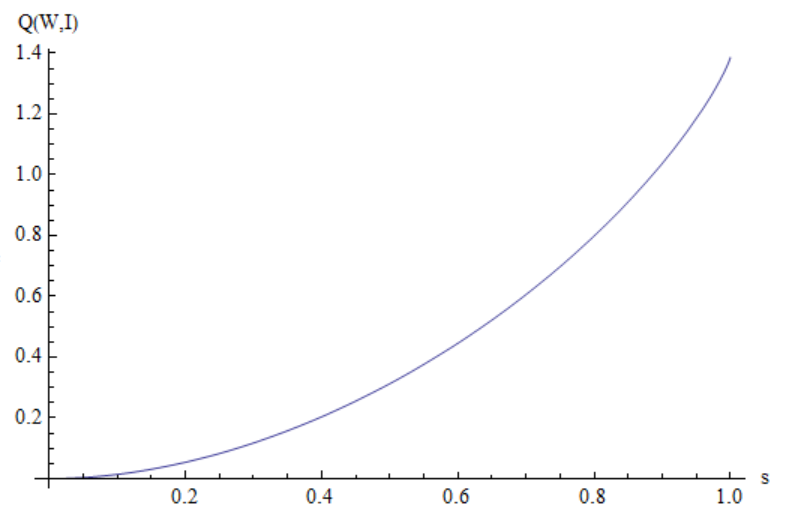
\includegraphics[scale=0.8]{figures/WIrelativecalc.png}
\caption{Plot of \eqref{hjreherjrie}.}
\label{figr5}
\end{center}
\end{figure}
\begin{equation}
Q(I_4 \| W)=\frac{1}{4} (-3 \log (1-s)-\log (3 s+1))
\label{dfsfsd}
\end{equation}
with its plot:
\begin{figure}[h]
\begin{center}
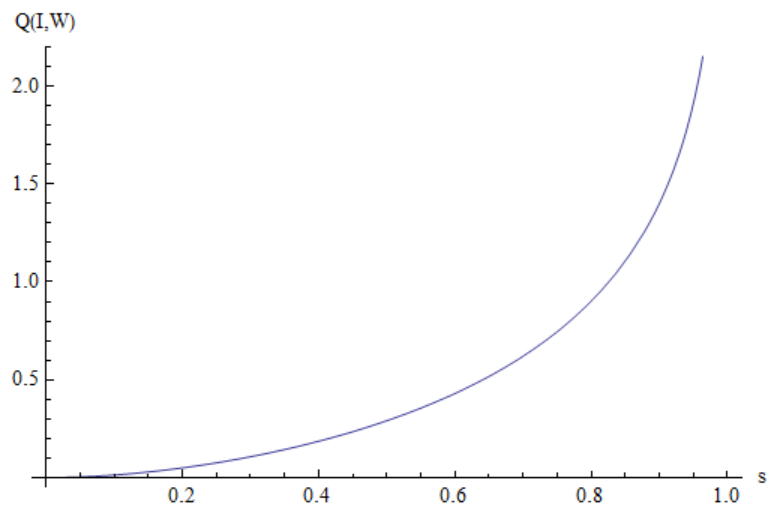
\includegraphics[scale=0.8]{figures/IWrelateivecalc.png}
\caption{The plot of \eqref{dfsfsd}.}
\label{figr6}
\end{center}
\end{figure}
\noindent
There is obvious asymmetry of the calculations however they have obvious qualitative commonalities.
\subsection{Mixed-Pure}
We now calculate the Relative entropy between the state $\sigma(\theta)$ of \eqref{sigmastate} and the Werner State \eqref{wernerstate} with $\ket{\Psi}=(\ket{00}+\ket{11})/\sqrt{2}$. We find that  
\begin{equation}
Q(\sigma\|W)=\frac{1}{2} \left(\log \left(\frac{16}{-3 s^2+2 s+1}\right)+\sin (2 \theta ) \log \left(\frac{1-s}{3 s+1}\right)\right)
\label{qentropy}
\end{equation}
with the plot:
\begin{figure}[H]
\begin{center}
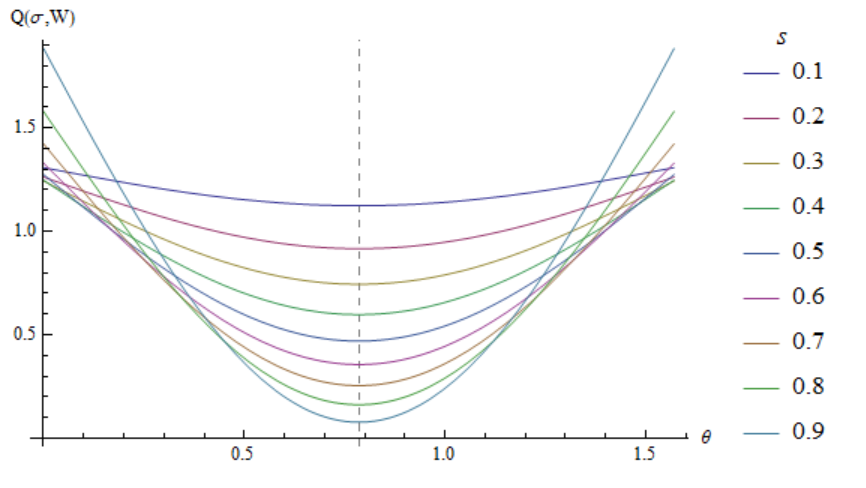
\includegraphics[scale=0.8]{figures/PureMixedRelativeEntropy.png}\caption{We can see that $Q(\sigma\|W)$ has an extremum for $s=0.5$ thus denoting that can be used as an entanglement measure.}
\label{figr7}
\end{center}
\end{figure}
\noindent
As we can see this measure of departure can detect the maximum entanglement of state $\sigma(\theta)$. This result might be useful in an experiment that can directly measure the quantum relative entropy.  We can easily check that $Q(W\|\sigma)$ diverges.
